\newpage
\section{Control Unit}
The Control Unit consists of the PSoC which converts the analogue inputs to digital values which can be handled by the GUI. This is done using the PSoC's internal ADCs. The noise in these converters can be lowered by connecting them to a \SI{100}{\nano \farad} capacitor. Furthermore, another \SI{100}{\nano \farad} is connected in parallel with the PSoC's positive power supply in order to remove potential ripple.

\begin{figure}[H]
	\centering
	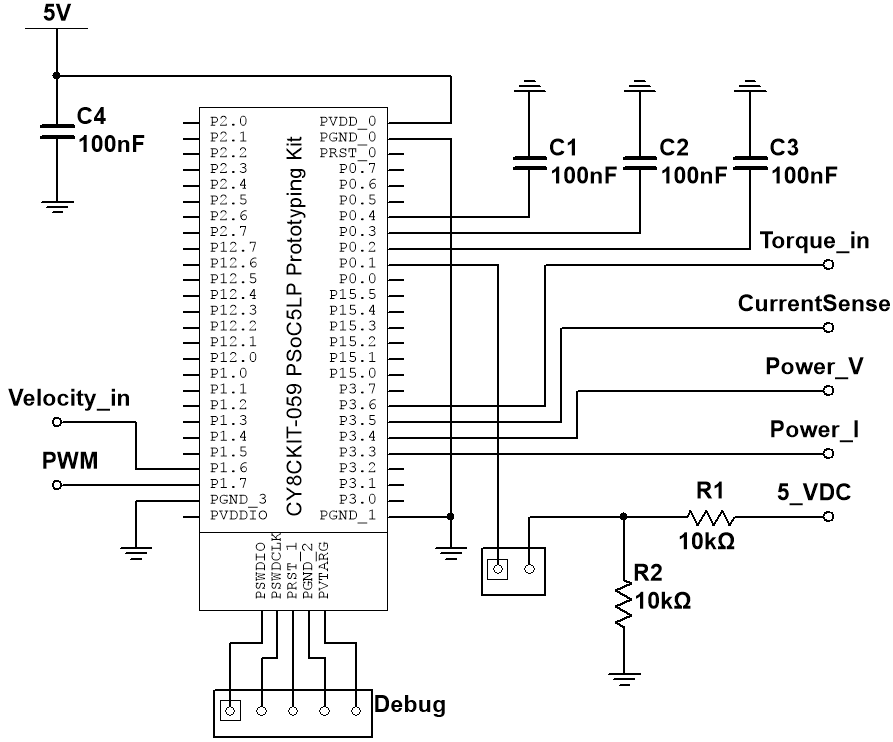
\includegraphics[width=0.8\linewidth]{Hardware/Pictures/PSoC}
	\caption{The hardware-configuration of the PSoC}
	\label{fig:PSoC_Hardware}
\end{figure}

The voltage-divider consisting of the resistors R1 and R2 gives and output-voltage of \SI{2.5}{\volt}. This reference-voltage isn't utilized on the current version of Rolling Road, but can be by connecting the two output harwin-pins with each other. This voltage is only added for future versions which might contain components which uses this voltage.

Five harwin-pins are added to the circuit which can be used to debug the PSoC, if the USB-connection isn't available. \fxnote{de bruges også til at programmere den - TN}